\section{Method}
\label{sec:method}

\subsection{Task and GRPO Training}
\label{sec:task}

Given premises $P_1,\ldots,P_k$ and conclusion $C$, the task is to produce a formal program $F=\{c_1,\ldots,c_n\}$ verified by an external solver $S\in\{\text{Prover9, SWI-Prolog}\}$.
We train with Group Relative Policy Optimization (GRPO)~\citep{deepseekmath} ($K{=}4$), where each rollout receives binary execution reward $r_{\text{exec}}(x) = \mathbf{1}[S(F_x){=}\textit{proved}]$.
This optimizes prove rate but provides no signal about \emph{component necessity} (Figure~\ref{fig:sta-overview}a): a formalization embedding the conclusion among its premises receives the same reward as a faithful derivation.
All experiments draw from FOLIO~\citep{folio}; the held-out evaluation set (100 examples) contains 34 True, 25 False, and 41 Unknown labels, with only True-labeled examples admitting valid proofs (theoretical PR ceiling ${\sim}34\%$).
Exec-only GRPO reaching $\text{PR}{=}93\%$ (\S\ref{sec:diagnostic}), nearly $3\times$ this ceiling, confirms the solver accepts formalizations for nominally unprovable examples, constituting direct evidence of structural gaming independent of ISR.

\subsection{Solver Trace Ablation (STA)}
\label{sec:sta}

\begin{figure*}[t]
\centering
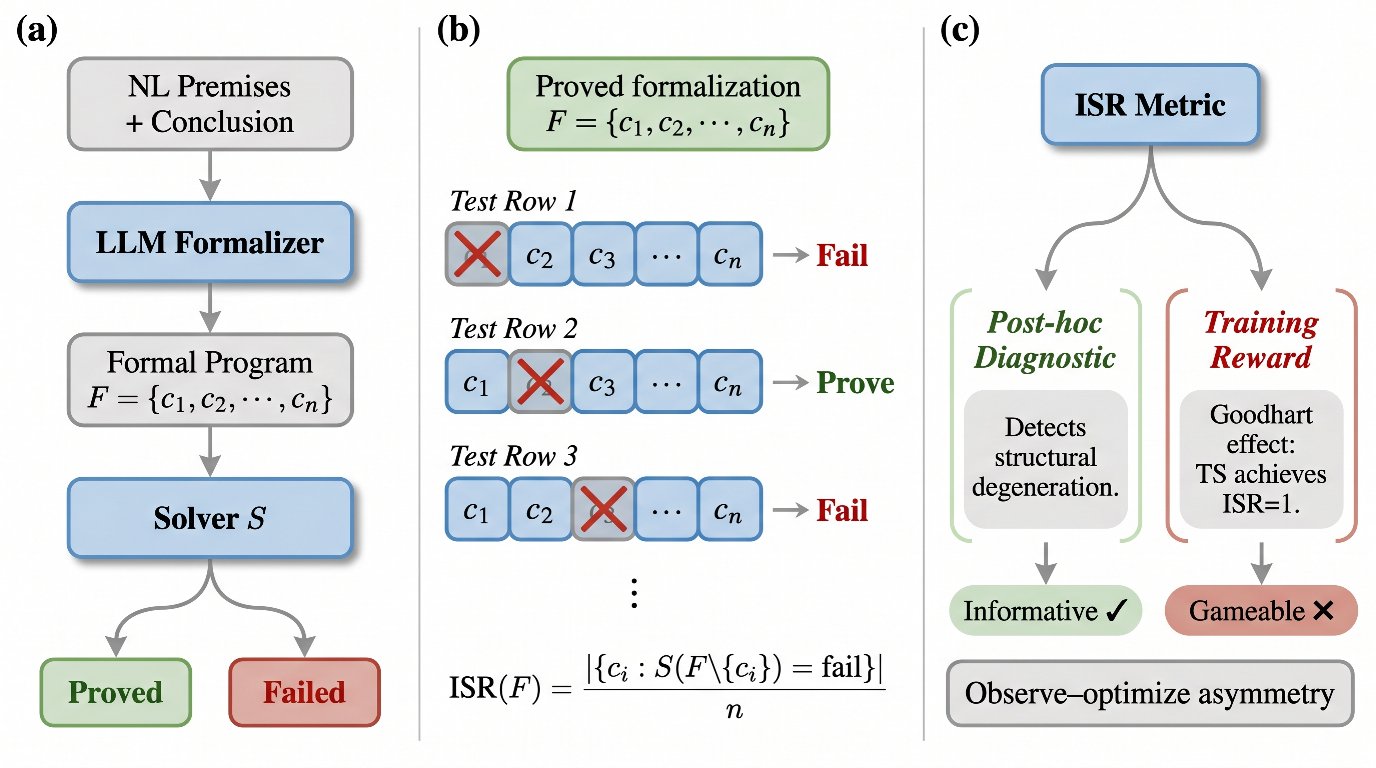
\includegraphics[width=\textwidth]{figures/fig1_sta_overview.pdf}
\caption{STA overview. \textbf{(a)}~The formalization pipeline: an LLM translates natural-language (NL) premises into formal logic, verified by an external solver. \textbf{(b)}~STA removes each component in turn and re-runs the solver; the fraction of necessary components yields ISR. \textbf{(c)}~Applied post-hoc, ISR detects structural hacking; repurposed as reward, it triggers a Goodhart effect where tautological shortcuts (TS) achieve $\text{ISR}{=}1$ by construction.}
\label{fig:sta-overview}
\end{figure*}

STA tests whether each component of a proved formalization is individually necessary for proof success (Figure~\ref{fig:sta-overview}; Algorithm~\ref{alg:sta}).
Given a proved $x$ with $n$ components, STA constructs $n$ ablated variants $x\setminus\{c_i\}$ and re-runs the solver (Algorithm~\ref{alg:sta}).
A component is \emph{necessary} if its removal causes proof failure.
What constitutes a component depends on the logic: premises in FOL, clauses or ground facts in Prolog.
LOO ablation itself is standard in mutation testing and sensitivity analysis~\citep{demillo1978, jia-harman-survey}; novelty lies in its application as a GRPO-hacking diagnostic and the empirical phenomena it surfaces.

\begin{algorithm}[t]
\caption{Solver Trace Ablation (STA)}
\label{alg:sta}
\begin{algorithmic}[1]
\REQUIRE Proved formalization $x = \{c_1, \ldots, c_n\}$, solver $S$
\ENSURE $\text{ISR}(x) \in [0, 1]$
\STATE $\textit{necessary} \gets 0$
\FOR{$i = 1$ to $n$}
    \IF{$S(x \setminus \{c_i\}) = \textit{failed}$}
        \STATE $\textit{necessary} \gets \textit{necessary} + 1$
    \ENDIF
\ENDFOR
\RETURN $\textit{necessary} \,/\, n$
\end{algorithmic}
\end{algorithm}

\paragraph{Intensional Structural Reward.}\footnote{Not \emph{intentional}; \emph{intensional} contrasts with extensional (execution-only) evaluation.}
For a proved formalization $x = \{c_1, \ldots, c_n\}$, ISR is the fraction of necessary components:
\begin{equation}
  \text{ISR}(x) = \frac{1}{n}\sum_{i=1}^{n}\mathbf{1}\bigl[S(x\setminus\{c_i\})=\textit{failed}\bigr]
  \label{eq:isr}
\end{equation}
ISR is defined only for proved formalizations: ISR${=}1$ means every component is necessary; ISR${=}0$ means complete redundancy.
An ISR of zero for proved samples can arise from structural degeneration or genuine redundancy; our hacking mode classification (\S\ref{sec:taxonomy-method}) disambiguates these cases, with ${>}90\%$ of low-ISR proved samples exhibiting identifiable hacking patterns.
ISR computes the LOO marginal contribution, a restriction of the Shapley value to the maximal coalition (Appendix~\ref{app:shapley}); full interaction detection would require $O(2^n)$ evaluations.
ISR quantifies component redundancy, not semantic faithfulness; its diagnostic value is realized through the downstream mode breakdown (\S\ref{sec:taxonomy}), not the scalar alone.
In practice, ISR serves as a screening trigger: anomalously low (or high) values flag samples for mode-level classification (\S\ref{sec:taxonomy-method}), which provides the definitive diagnostic.
We report \emph{proved-only} ISR (denoted ISR$^*$) throughout to avoid conflating component necessity with prove rate.

\paragraph{LOO independence assumption.}
LOO ablation tests individual, not joint, component necessity~\citep{jia-harman-survey}, systematically underestimating ISR when jointly-necessary components exist; the observed collapse is therefore conservative.

\subsection{Reward Conditions and Hacking Modes}
\label{sec:rewards}
\label{sec:taxonomy-method}

We study six conditions: exec-only ($r_{\text{exec}}$), ISR low/high-dose ($r_{\text{exec}}\cdot(1{+}\beta\,\text{ISR})$ at $\beta\in\{0.1,0.3\}$), matched random controls ($r_{\text{exec}}\cdot(1{+}\beta u)$, $u\sim\mathcal{U}(0,1)$), and a supervised fine-tuning (SFT) baseline (negative log-likelihood on gold formalizations).
Multiplicative bonuses apply only to proved samples, keeping the prove-rate floor intact.
Random isolates ISR-specific signal from generic reward-variance effects; SFT isolates whether structural degeneration arises from RL optimization or data exposure alone.
Each RL condition uses seeds $\{42,43,44\}$ and identical training data (formulation alternatives in Appendix~\ref{app:setup}).

\begin{table*}[t]
\centering
\small
\begin{tabular}{lcccccc}
\toprule
\textbf{Condition} & $\boldsymbol{\beta}$ & \textbf{PR\%}$\uparrow$ & \textbf{ISR}$^*$ & \textbf{TS\%} & \textbf{CE\%} & \textbf{N-H\%} \\
\midrule
Base (0-shot) & --- & 12 & --- & --- & --- & --- \\ %% registry: sta-phase0-baseline
SFT & --- & 13 & 0.595 & 0 & 8 & \textbf{92} \\ %% registry: plan009-sft-baseline-s42-1000/s43-1000/s44-1000-r3 (3-seed pooled)
\midrule
Exec-only$^\dagger$ & --- & 93 & 0.132 & 0 & 87 & 8 \\ %% registry: plan001-exec-only-s42-r2 (PG corrected)
ISR (3-seed) & 0.1 & 77{\scriptsize$\pm$14} & $1.06\times^\ddagger$ & \textbf{71}$^\P$ & 18 & 6 \\ %% registry: plan002-additive-b01-s42/s43-r2/s44 (pooled, D095 FINAL)
ISR (5-seed) & 0.1 & 70{\scriptsize$\pm$19} & (0.63)$^\ddagger$ & 54 & 18 & 23 \\ %% registry: plan002-additive-b01-s42--s46 (pooled)
Random & 0.1 & \textbf{87}{\scriptsize$\pm$8} & 0.117{\scriptsize$\pm$.04} & 14$^\S$ & 69 & 10 \\ %% registry: plan018-additive-random-b01-s42/s43-r3/s44-r2 (D095 FINAL)
Shuffled-ISR & 0.1 & 15{\scriptsize$\pm$1} & 0.559{\scriptsize$\pm$.02} & 7 & 7 & \textbf{87} \\ %% registry: d157-shuffled-isr-s42-r3/s43/s44 (3-seed pooled, D159)
\midrule
ISR & 0.3 & 66{\scriptsize$\pm$42} & 0.39{\scriptsize$\pm$.31} & \textbf{50} & 37 & 11 \\ %% registry: plan002-additive-b03-s42, exp1-isr-b03-s43-r3, plan002-additive-b03-s44 (pooled; D106 s43 genuine 23→20)
Random & 0.3 & 54{\scriptsize$\pm$35} & 0.09{\scriptsize$\pm$.09} & 7 & 91 & 2 \\ %% registry: plan017-additive-random-s42, exp1-random-b03-s43-r4, exp1-random-b03-s44-r2 (pooled; D086 TS: s42=4,s43=7,s44=0)
\bottomrule
\end{tabular}
\caption{Goodhart landscape across reward conditions. PR = prove rate; ISR$^*$ = proved-only ISR; TS = tautological shortcut; CE = conclusion embedding; N-H = non-hacking (upper bound on genuine reasoning). Multi-seed rows: pooled TS/CE/N-H; PR/ISR$^*$ as mean$\pm$std. $^\dagger$Seed~42 only. $^\ddagger$Premise-count-matched (\S\ref{sec:goodhart}). $^\P$FN-corrected (\S\ref{app:h8}). $^\S$Seed-dependent (s43: 38.3\%). Per-seed data: Table~\ref{tab:fol-detailed}.}
\label{tab:goodhart-landscape}
\end{table*}

\paragraph{Hacking taxonomy.}
Across conditions, seeds, and logic types we identify eight structural-degeneration modes (full definitions in Appendix~\ref{app:hacking-modes}), dominated by three: \textbf{CE} (conclusion embedded among multiple premises), \textbf{TS} (single-premise conclusion duplication; targets ISR directly since removing the sole premise forces $\text{ISR}\geq 0.5$), and \textbf{PG} (premise-subset gaming: each component is LOO-necessary but the premise set is incomplete; Appendix~\ref{app:h8}).
Five additional modes (tautological collapse, repetition, complexity-without-utility, contradiction explosion, and query-as-fact [Prolog-specific]) appear in specific seeds or conditions.
CE and TS are robust across conditions and seeds; the remaining five modes are configuration-specific observations whose generalizability requires further investigation.
Modes are identified by strict text matching (CE/TS) plus functional analysis of the per-sample $n_{\text{necessary}}$ distribution; when patterns overlap, we assign the most specific mode (PG $>$ CE $>$ TS).
The non-hacking rate is an upper bound on genuine reasoning.

Low ISR signals redundancy under exec-only but metric gaming under ISR-as-reward; the mode breakdown, not the ISR scalar, licenses interpretation.
